%%%%%%%%%%%%%%%%%%%%%%%%%%%%%%
%%                                                     %%
%%   LaTeX template voor P&O: Computerwetenschappen.   %%
%%                                                     %%
%%   Schrijfopdracht 1                                 %%
%%                                                     %%
%%   7 oktober 2013                                    %%
%%   Versie 1.1                                        %%
%%                                                     %%
%%%%%%%%%%%%%%%%%%%%%%%%%%%%%%

\documentclass{peno-opdracht1}
\usepackage{comment}
\usepackage{pdfpages}
\usepackage{titlesec}
\usepackage{textcomp}
\usepackage{sidecap}
\usepackage{caption}
\usepackage{scrextend}
\titleformat{\section}
{\normalfont\fontsize{12}{15}\bfseries}{\thesection}{1em}{}

\team{Zilver} % teamkleur

\begin{document}

\maketitle

\noindent
	Ons team bestaat uit Bram Vandendriessche, Matthias Van der Heyden, Jef Versyck, Vincent Vliegen, Arne Vlietinck en Laura Vranken. Bram werd aangeduid als CEO en Arne zal de taak van CAO op zich nemen. \\
	Om op een effici\"ente manier het geheel te kunnen realiseren, wordt het team in twee verdeeld. De ene groep (Bram, Jef en Arne) buigt zich over het virtual testbed. Het andere team  (Matthias, Vincent en Laura) zorgt voor de drone autopilot.\\
	Een gedetailleerde planning kan teruggevonden worden in appendix \ref{App:Planning}.

\section{API keuze}
Als API voor het generen van 3D-beelden zijn er drie kandidaten: Blender, JMonkeyEngine en OpenGL.\\
Blender heeft als voordeel dat voorwerpen gemakkelijk gegeneerd kunnen worden door de gebruiksvriendelijke interface. Daarnaast moet er voor Blender kennis zijn van Python, aan deze voorwaarde voldoet niet iedereen. Ook wordt er hierdoor een extra moeilijkheid gecre\"eerd, namelijk de \mbox{communicatie} tussen JAVA en Python. Vooral door deze laatste eigenschap zal er geen gebruik gemaakt worden van Blender. \\
JMonkeyEngine is gebruiksvriendelijker dan OpenGL, maar door gebrek aan uitgebreide communities wordt er niet voor geopteerd.\\
Onze keuze gaat uit naar OpenGL ondanks dat alles gecodeerd moet worden. Toch kan dit deels omzeild worden door figuren te importeren vanuit Blender. Deze optie zal dan ook gebruikt worden. 

\section{Autopilot}
De drone autopilot moet zijn positie tegenover het doel kunnen bepalen aan de hand van twee gekregen camerabeelden. Eerst wordt de diepte bepaald op basis van de brandpuntsafstand, de afstand tussen de zichtbare rode bol op het frame en het middelpunt van het frame (in pixels) en de afstand tussen de camera\textquotesingle s (in meter).\footnote{Deze formule en de grafische weergave kan teruggevonden worden op: (NASA tech briefs : A Guide to Stereovision and 3D Imaging, http://www.techbriefs.com/component/content/article/14925, geraadpleegd op: 5/10/2016.)\label{refnote}} Zie appendix \ref{App:Afstand}. \\
Om te vliegen, ori\"enteren we eerst de drone naar het doel. Hiervoor moet er opeenvolgend de bewegingen pitch, roll en yaw onder een bepaalde hoek uitgevoerd worden. Deze hoeken kunnen worden opgevraagd uit de interface. Vervolgens wordt naar het doel toegevlogen via een combinatie van thrust en pitch.
Deze berekeningen worden na iedere draai of na een bepaalde vliegafstand telkens opnieuw uitgevoerd.
Als pixel waarop de berekeningen gebaseerd worden, kiezen we de pixel die het zwaartepunt van de gedetecteerde vorm weerspiegelt. Dit zwaartepunt bepalen we door de coördinaten van alle rode pixels op te slaan en hieruit de gemiddelde x- en y-co\"ordinaat te berekenen.

\section{GUI}
De GUI zal gezamenlijk gemaakt worden, zodanig de vereisten van beide subgroepen verwerkt kunnen worden. \\

\newpage
\appendix
\section{Gantt chart} \label{App:Planning}

\begin{figure}[h!]
	\begin{center}
		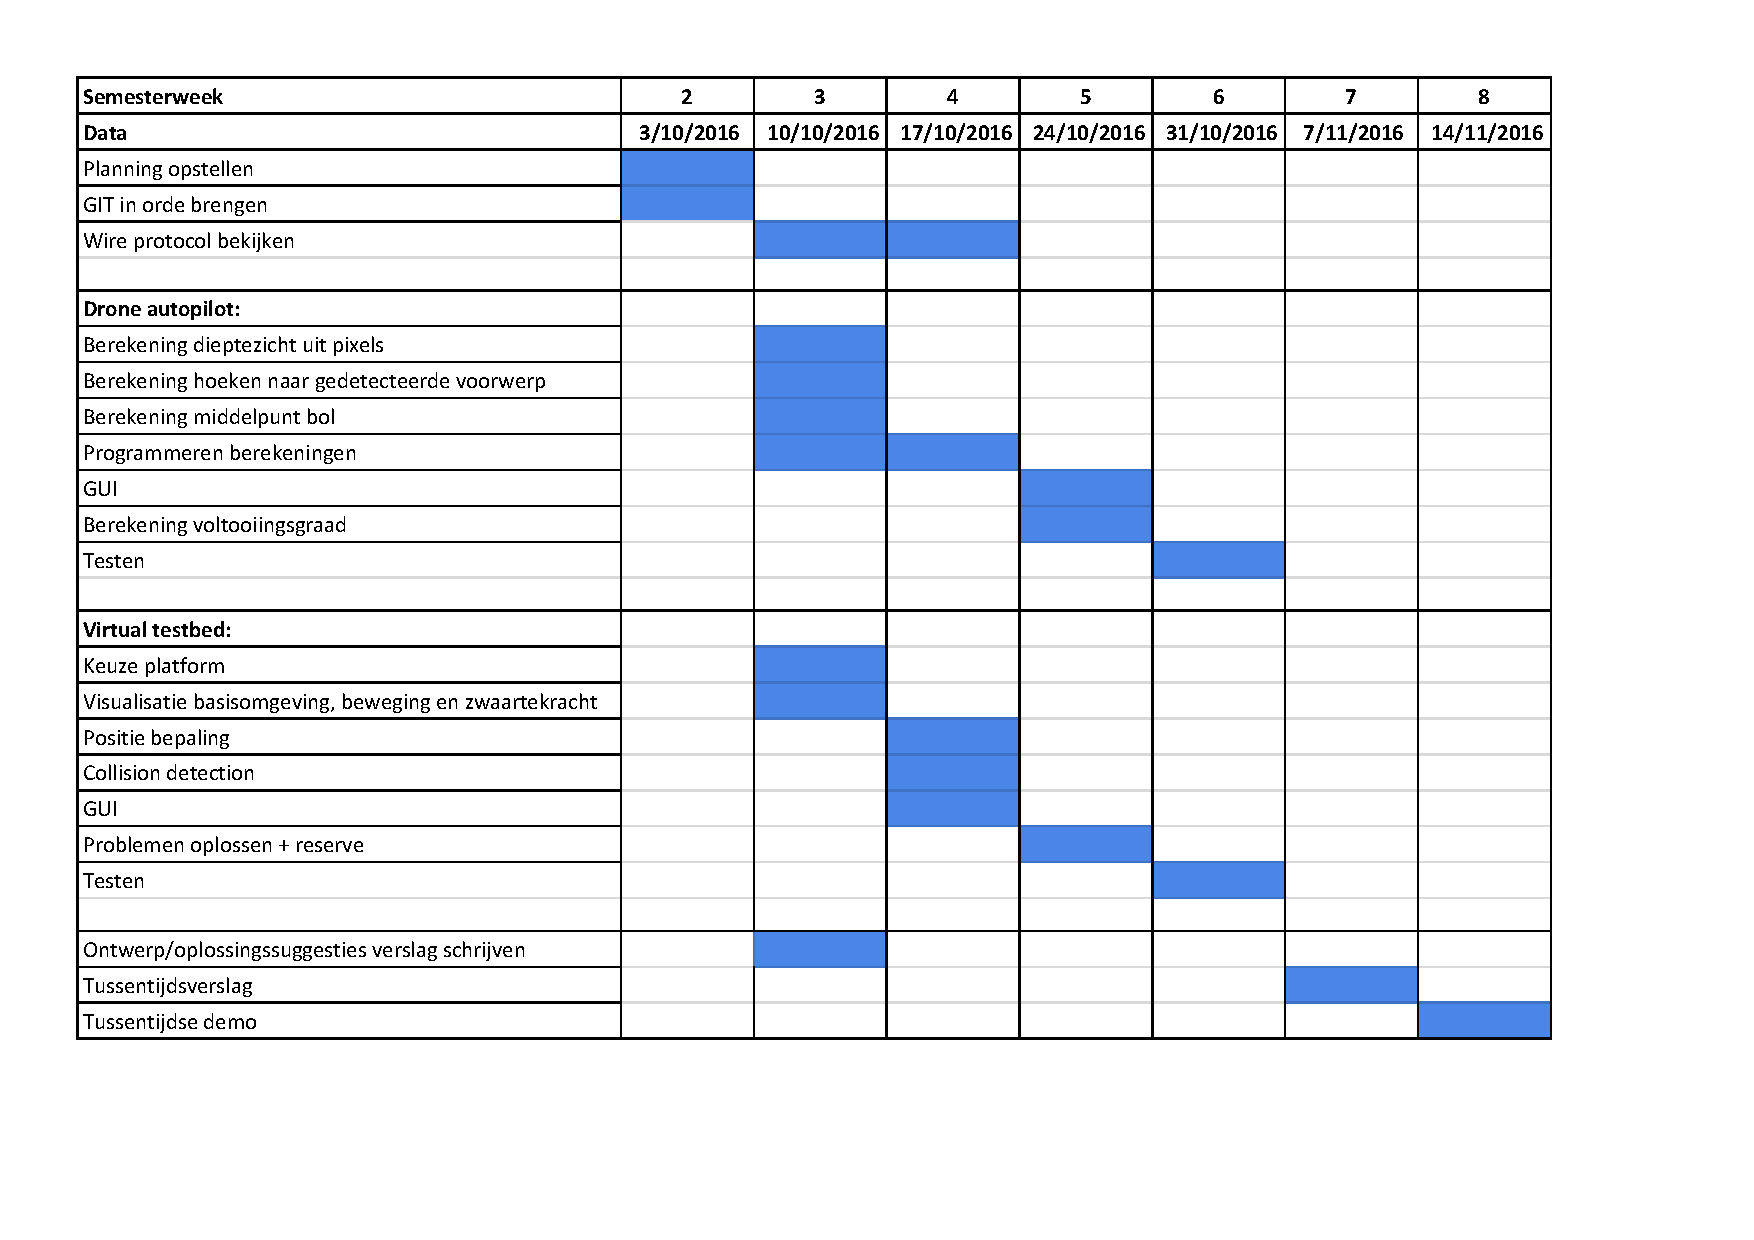
\includegraphics[scale=0.55]{Planning.pdf}
	\end{center}
\end{figure}

\section{Diepte-berekening} \label{App:Afstand}

\begin{figure}[h!]
	\begin{center}
		
		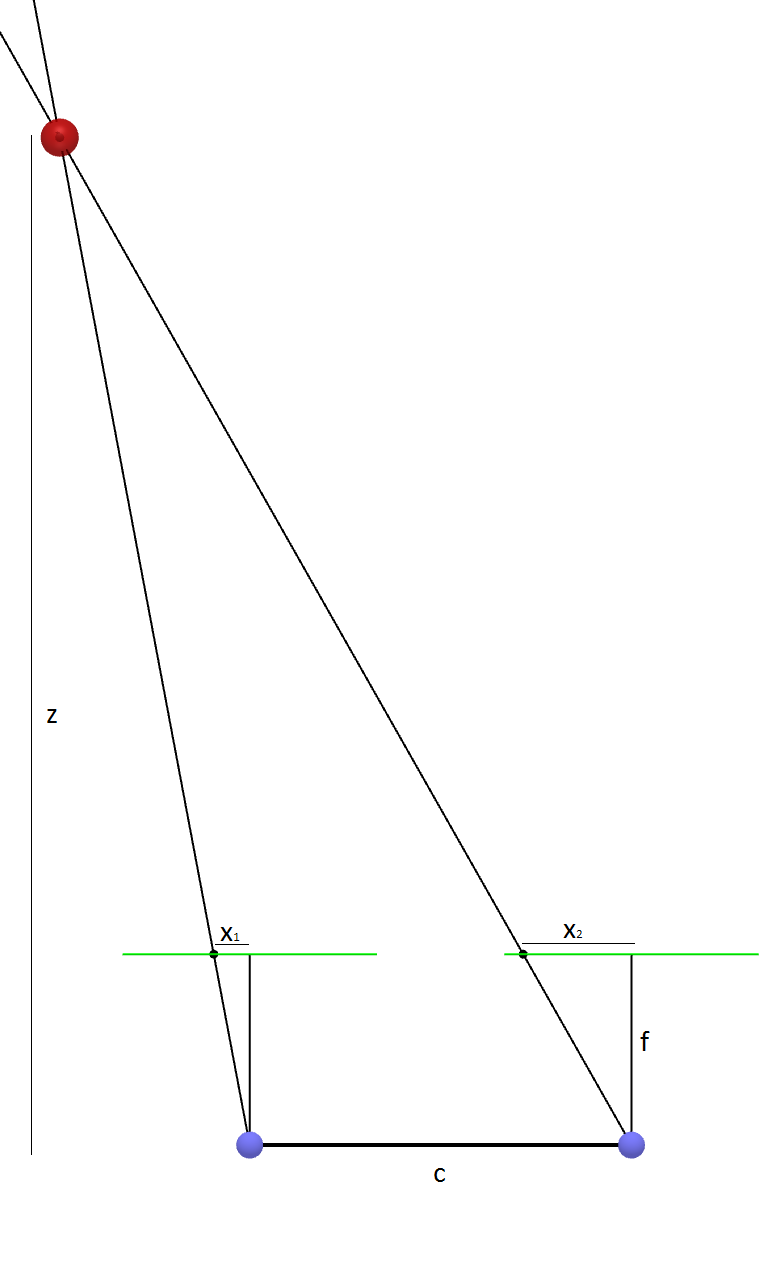
\includegraphics[scale=0.35]{Afstanden.png}
		\caption*{\(z = \frac{c \cdot f}{x_1 - x_2}\)}
	\end{center}
\end{figure}




3\end{document}
